\documentclass[10pt]{beamer}
\usetheme{Malmoe}
\usepackage[utf8x]{inputenc}
\usepackage{ucs}
\usepackage[english,russian]{babel}
\usepackage[OT1]{fontenc}
\usepackage{amsmath}
\usepackage{amsfonts}
\usepackage{amssymb}
\usepackage{graphicx}

\author{I.D. Tretyak$^{2,1}$, G.S. Goyman$^{1}$, V.V. Shashkin$^{1}$}
\title[SBP-SАT methods on grids with local refinement]{SBP-SAT approach for horizontal approximation of atmospheric dynamics equations on grids with local space refinement}
\setbeamercovered{transparent}
\setbeamertemplate{navigation symbols}{} 
\logo{
\includegraphics[width=0.9cm]{./images/logo.png}} 
\institute{Marchuk Institute of Numerical Mathematics RAS$^1$\\
National Research University <<Moscow Institute of Electronic Technology>>$^2$} 
%\date{} 
\subject{} 

\defbeamertemplate*{footline}{shadow theme}
{%
\leavevmode%
\hbox{\begin{beamercolorbox}[wd=.5\paperwidth,ht=2.5ex,dp=1.125ex,leftskip=.3cm plus1fil,rightskip=.3cm]{author in head/foot}%
\usebeamerfont{author in head/foot}\insertframenumber\,/\,\inserttotalframenumber\hfill\insertshortauthor
\end{beamercolorbox}%
\begin{beamercolorbox}[wd=.5\paperwidth,ht=2.5ex,dp=1.125ex,leftskip=.3cm,rightskip=.3cm plus1fil]{title in head/foot}%
\usebeamerfont{title in head/foot}\insertshorttitle%
\end{beamercolorbox}}%
\vskip0pt%
}
\begin{document}

\begin{frame}
\titlepage
\end{frame}



\begin{frame}{Introduction}

Methods of increasing detalization of atmosphere state forecast:

1. Increasing resolution globally 

\begin{enumerate}
\item[+] Improving effective resolution
\item[--] Rapid growth of required computing resources
\end{enumerate}

2. Local refinement of computational grid

\begin{enumerate}
\item[+] Saving computing resources
\item[+] Increasing the effective resolution in the refinement region
\item[--] Numerical errors at domains boundaries
\end{enumerate}
\end{frame}



\begin{frame}{Shallow water equations}
\textbf{Vector-invariant form of shallow water equations:}
$$
\begin{cases}
\frac{\partial \textbf{v}}{\partial t} = -(\xi+f)\textbf{k} \times \textbf{v}-\nabla(gh+K)\\
\frac{\partial h}{\partial t} = -\nabla \cdot (\textbf{v}h)
\end{cases}
$$

$\textbf{v} - $ horizontal velocity vector, $h$ - thickness of the fluid layer, $\textbf{k}$ - vertical unit vector, $\xi = \textbf{k} \cdot \nabla \times \textbf{v}$ - relative vorticity, $f$ - Coriolis parameter, $K=\textbf{v}\cdot \textbf{v} \slash 2$ - kinetic energy density.

\end{frame}



\begin{frame}{Computational grid}

\begin{figure}[h]
\centering
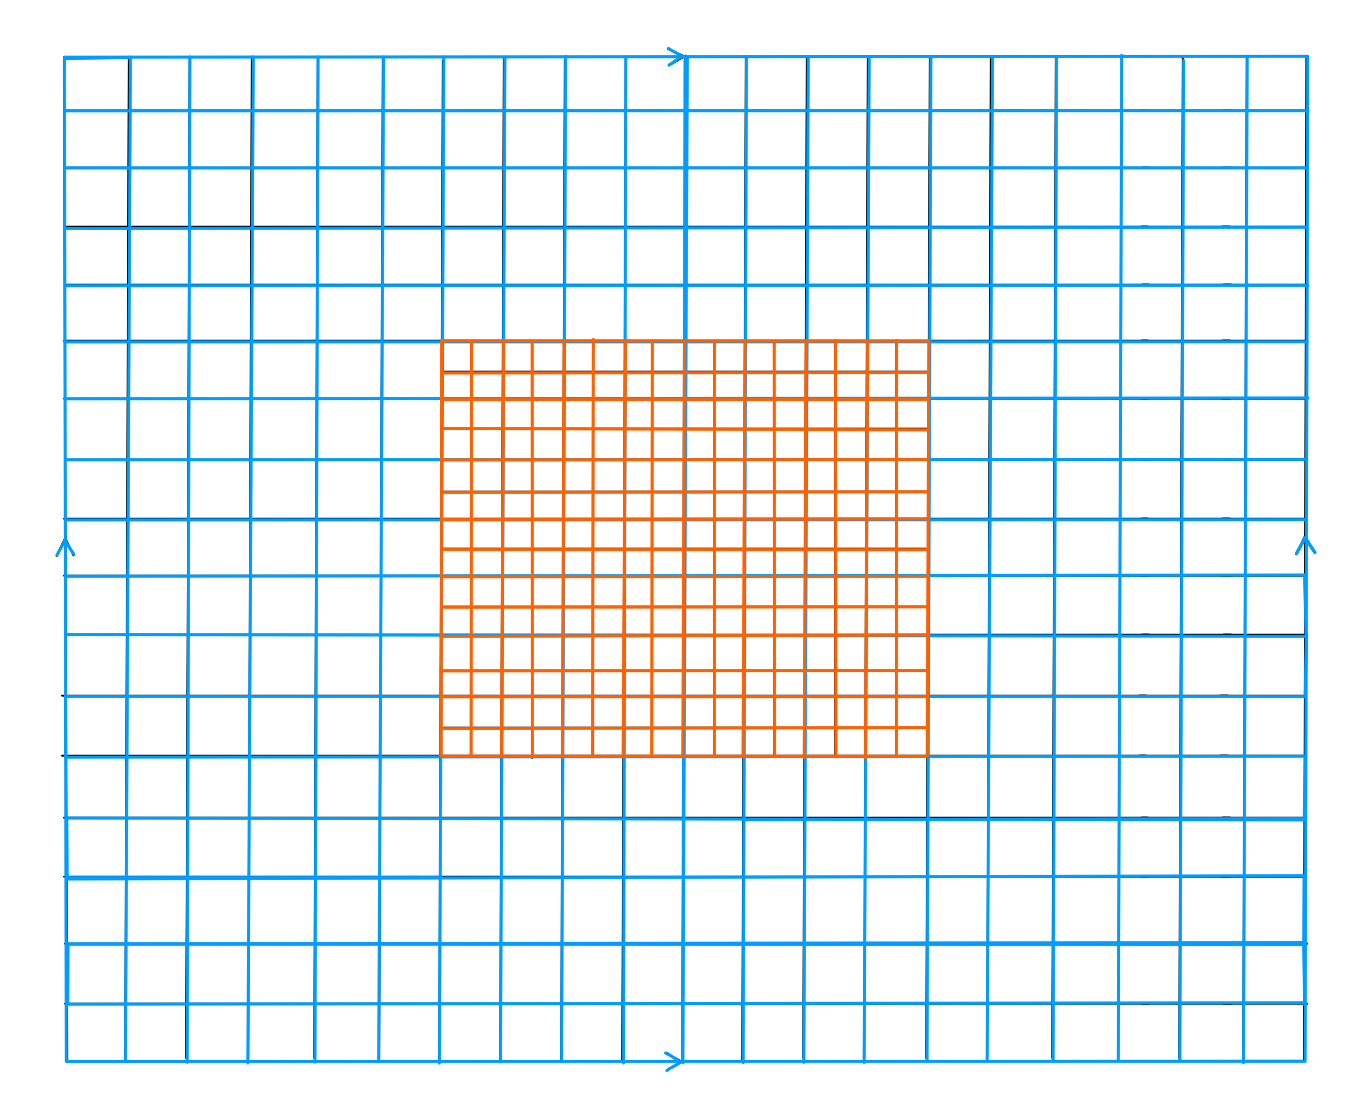
\includegraphics[width=0.8\linewidth]{./images/domain.png}
\caption{Possible configuration of the computational grid: biperiodic boundary conditions, a block with a local refinement of 2 times in the middle.}
\label{fig:mpr}
\end{figure}

\end{frame}



\begin{frame}{(SBP) Summation-by-parts finite differences}
$$\frac{\partial U}{\partial x}\approx D\textbf{u}$$

\textbf{Summation-by-parts (SBP):}
$$\textbf{u}^T HD \textbf{v} = (u_N v_N - u_0 v_0) -(D\textbf{u})^T H \textbf{v}$$

Discrete analogue of integration-by-parts (IBP):
$$\int\limits_{a}^bU(x)\frac{\partial V(x)}{\partial x}=U(b)V(b)-U(a)V(a)-\int\limits_{a}^b {V(x)\frac{\partial U(x)}{\partial x}}$$

\begin{enumerate}
 \item Discrete analogues of mass and energy conservation laws performed.
 \item Stability theorem for linearized problem.
\end{enumerate}
\end{frame}


\begin{frame}{(SAT) Simultaneous Approximation Terms}
\textbf{Weak form of continuity conditions}
SAT-terms:
$$\frac{\partial U}{\partial x}\approx D\textbf{u} + SAT_0 + SAT_N,$$

$$SAT_0=\sigma_0 (\Delta u^{left}), \ SAT_N=\sigma_N(\Delta u^{right})$$

Weights $\sigma_0, \sigma_N$ are selected based on global SBP property requirement (global energy conservation).

\begin{figure}[h]
\centering
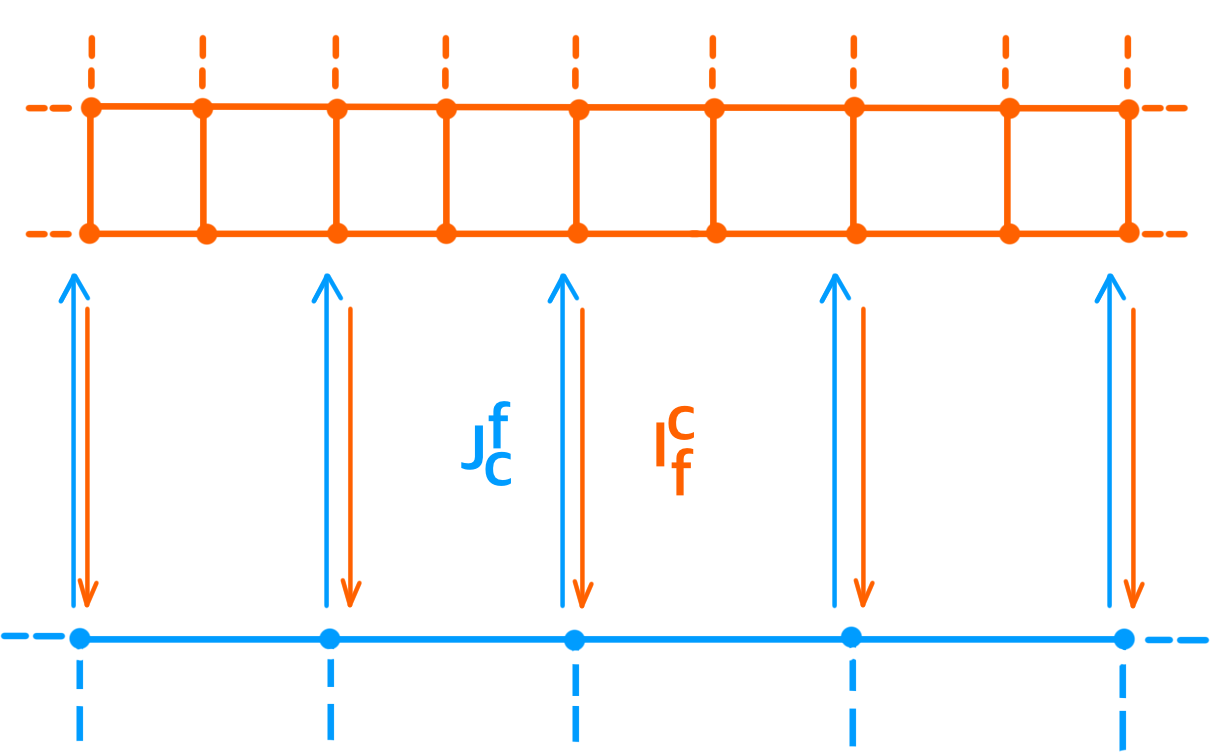
\includegraphics[width=0.5\linewidth]{./images/interp.png}
\caption{Interpolation between blocks with different resolutions}
\label{fig:mpr}
\end{figure}

\end{frame}




\begin{frame}{Kelvin-Helmholtz instability}

\begin{figure}[h]
\centering
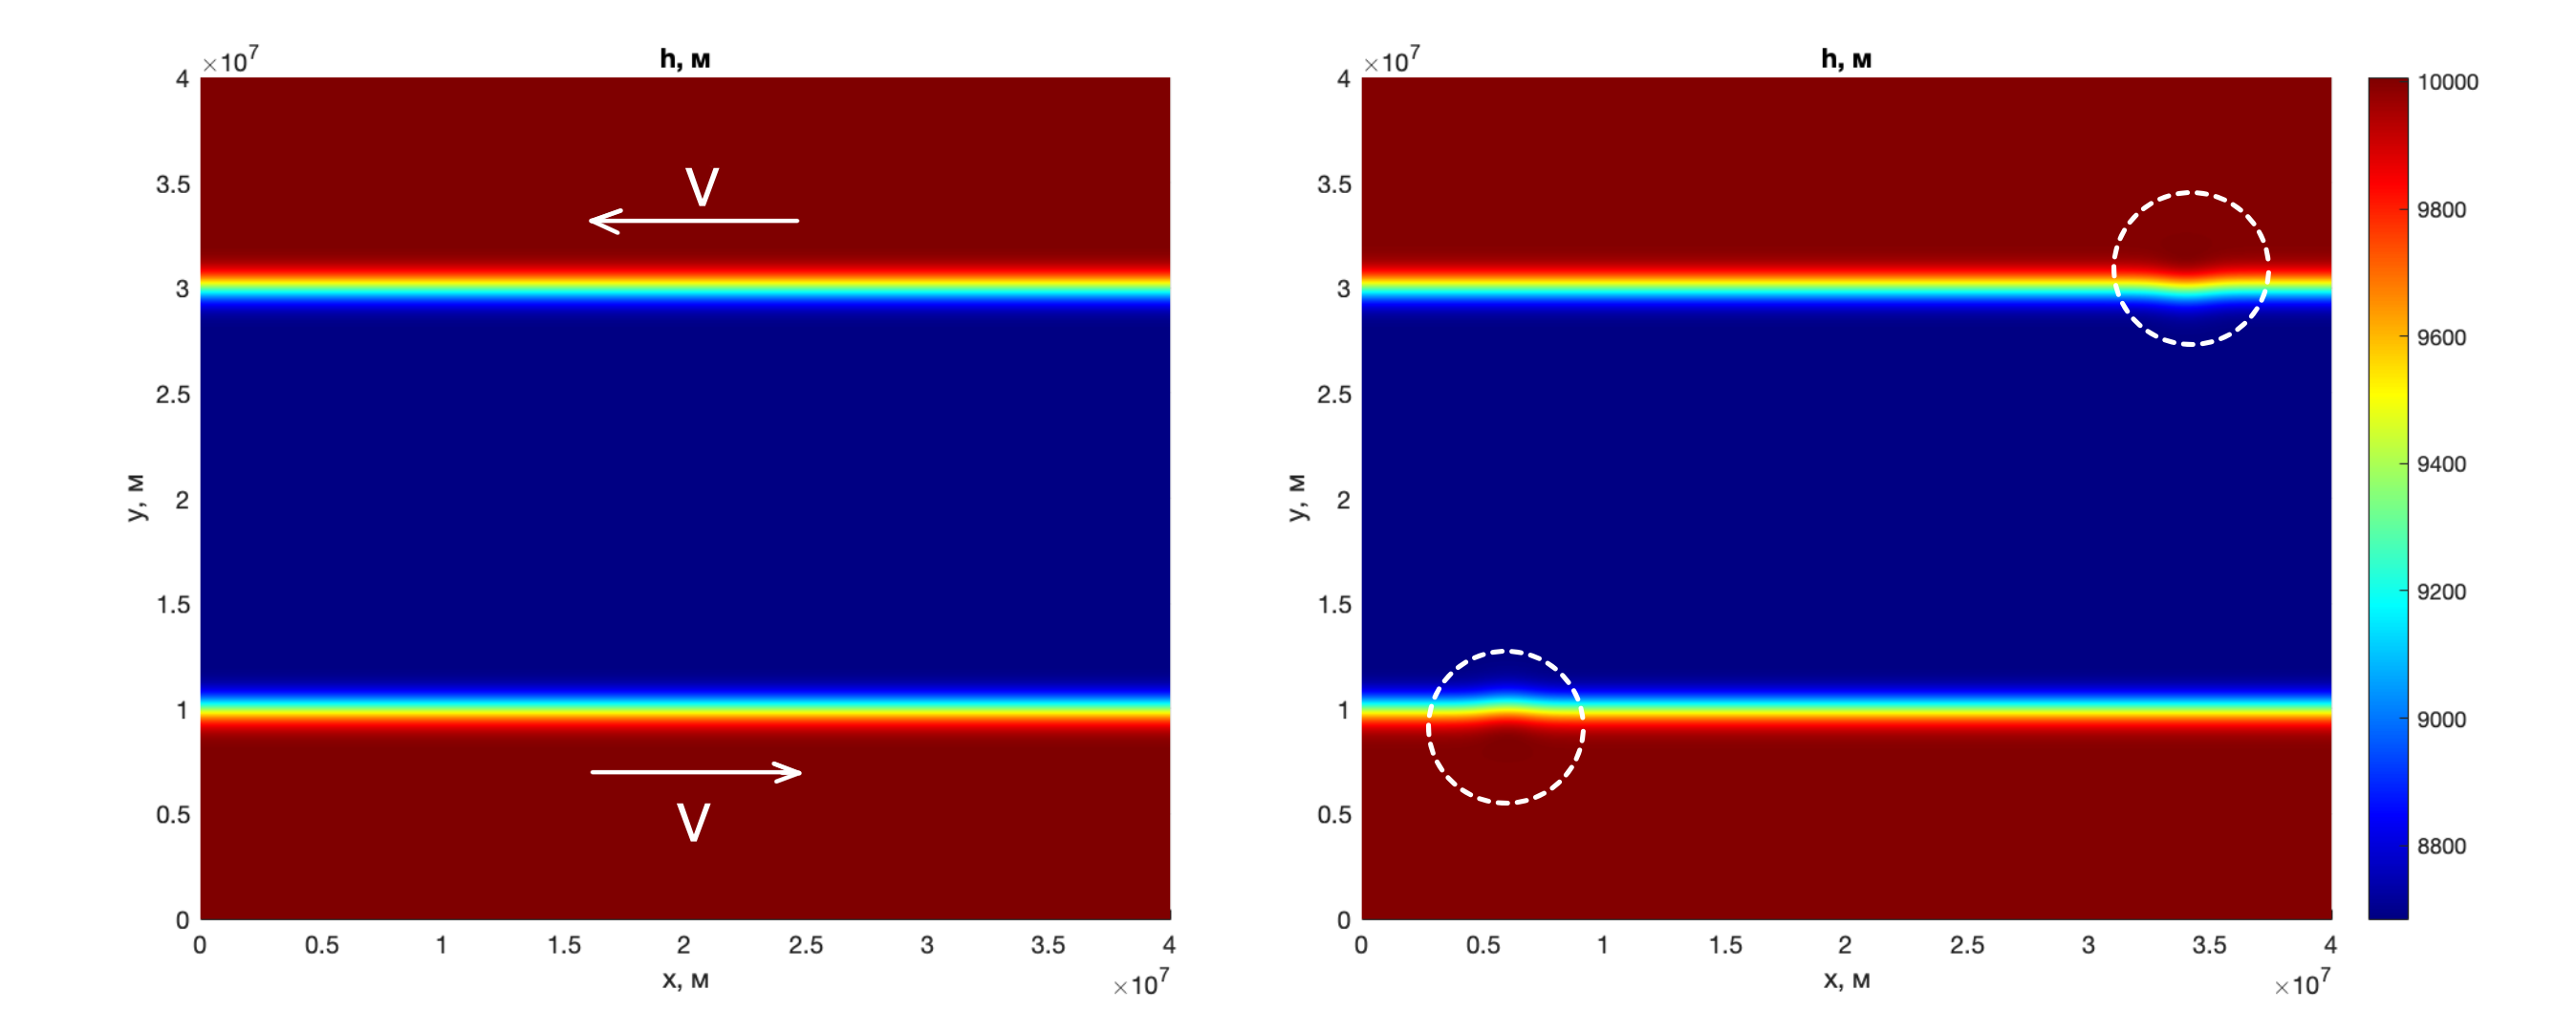
\includegraphics[width=1\linewidth]{./images/initial_cond_kelhelm.png}
\caption{Initial conditions for fluid layer thickness field -- h}
\label{fig:mpr}
\end{figure}

\end{frame}

\begin{frame}{Kelvin-Helmholtz instability}
\begin{figure}[h]
\centering
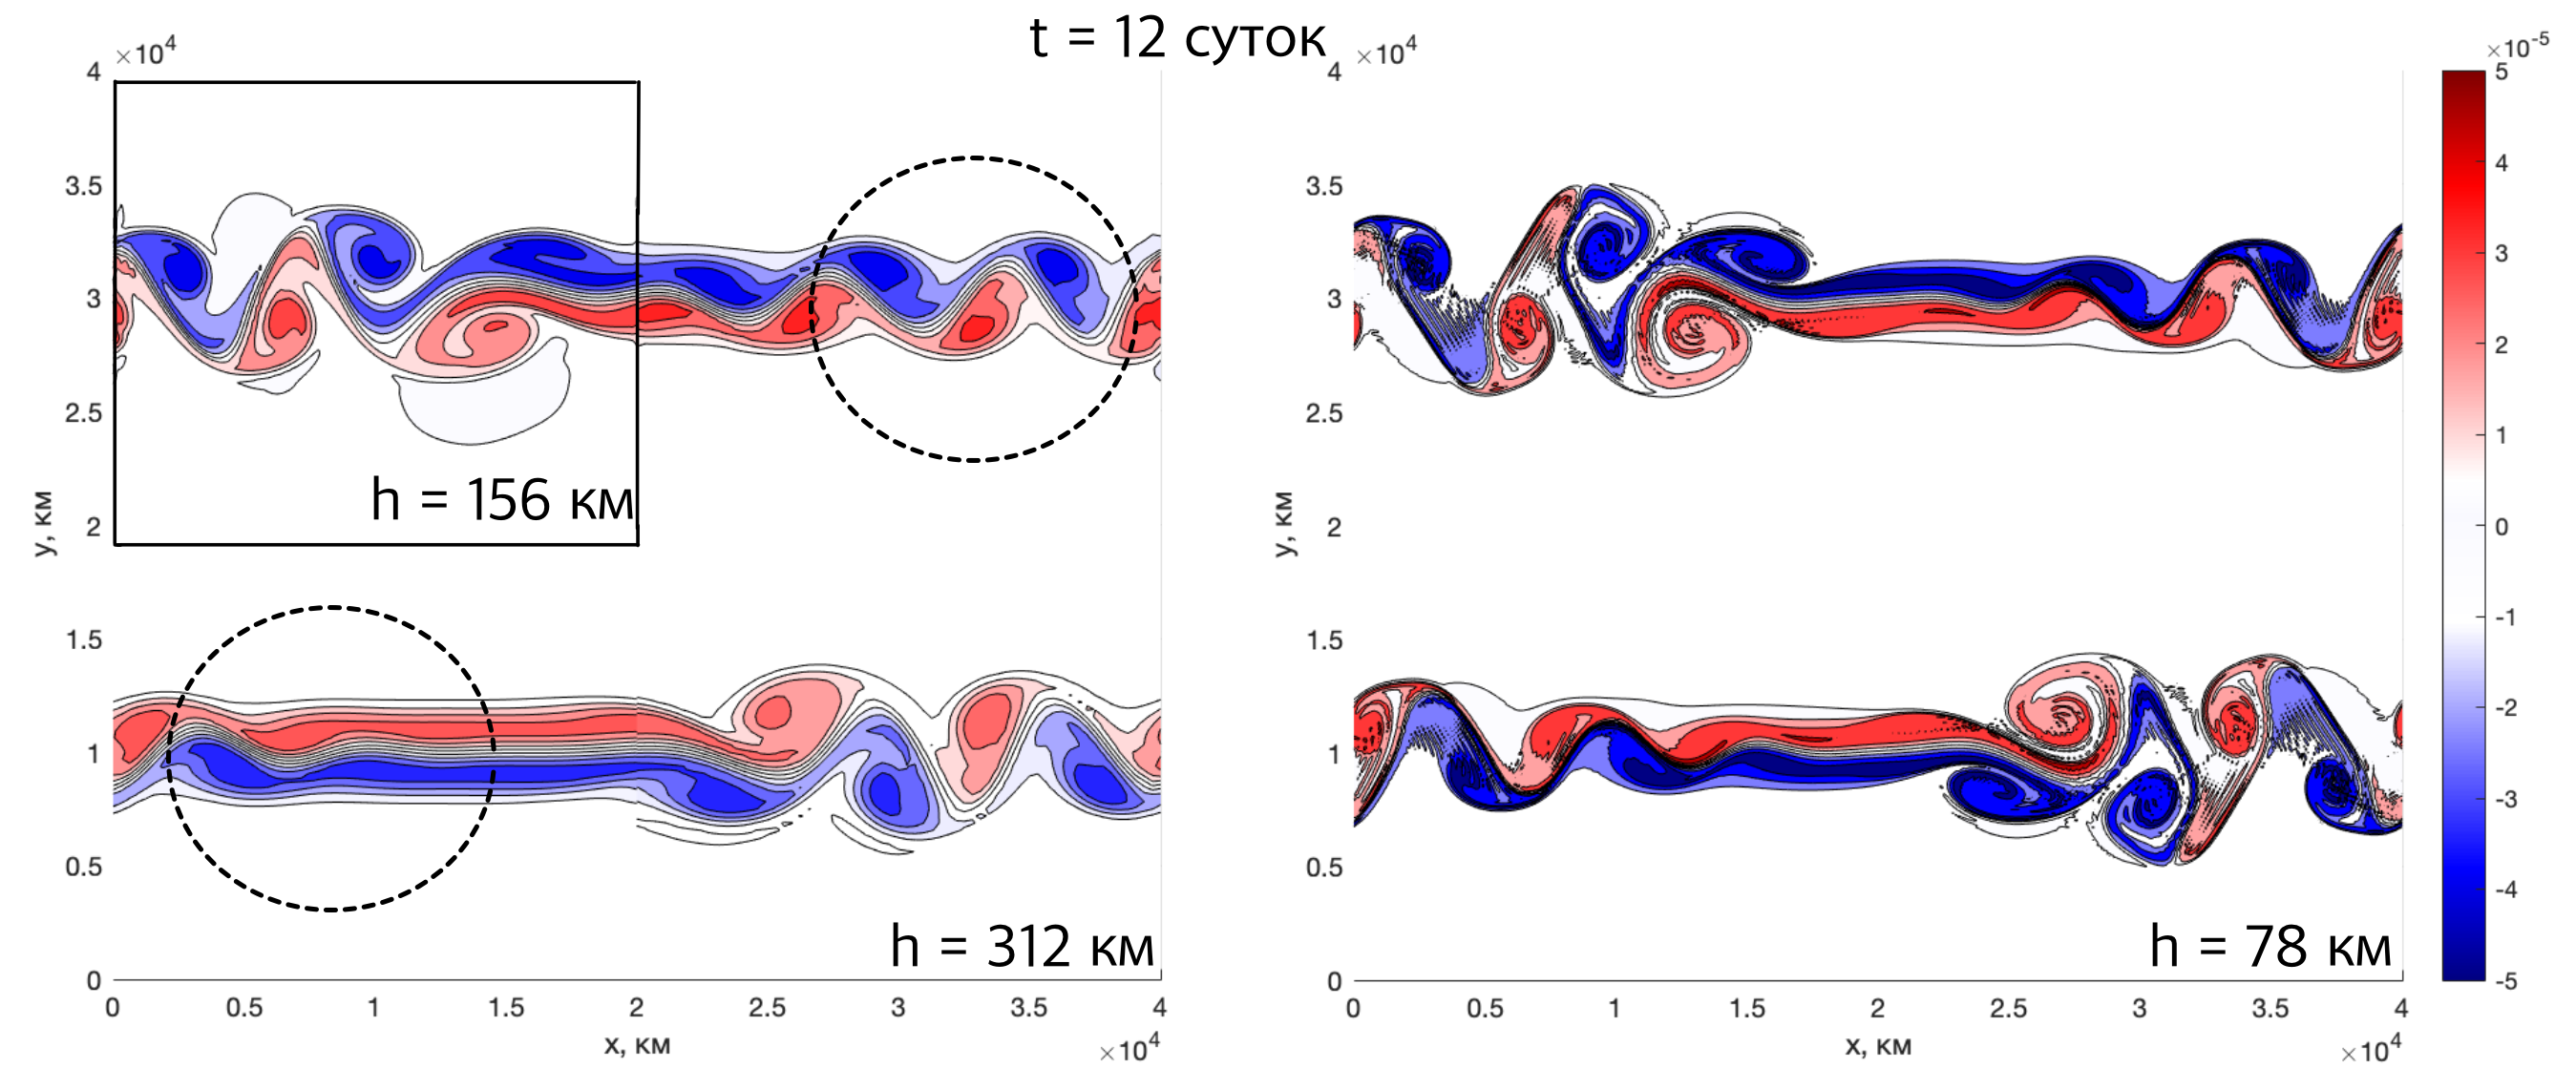
\includegraphics[width=1\linewidth]{./images/kelhelm12.png}
\caption{Relative vorticity field after 12 days}
\label{fig:mpr}
\end{figure}
\end{frame}

\begin{frame}{Kelvin-Helmholtz instability}
\begin{figure}[h]
\centering
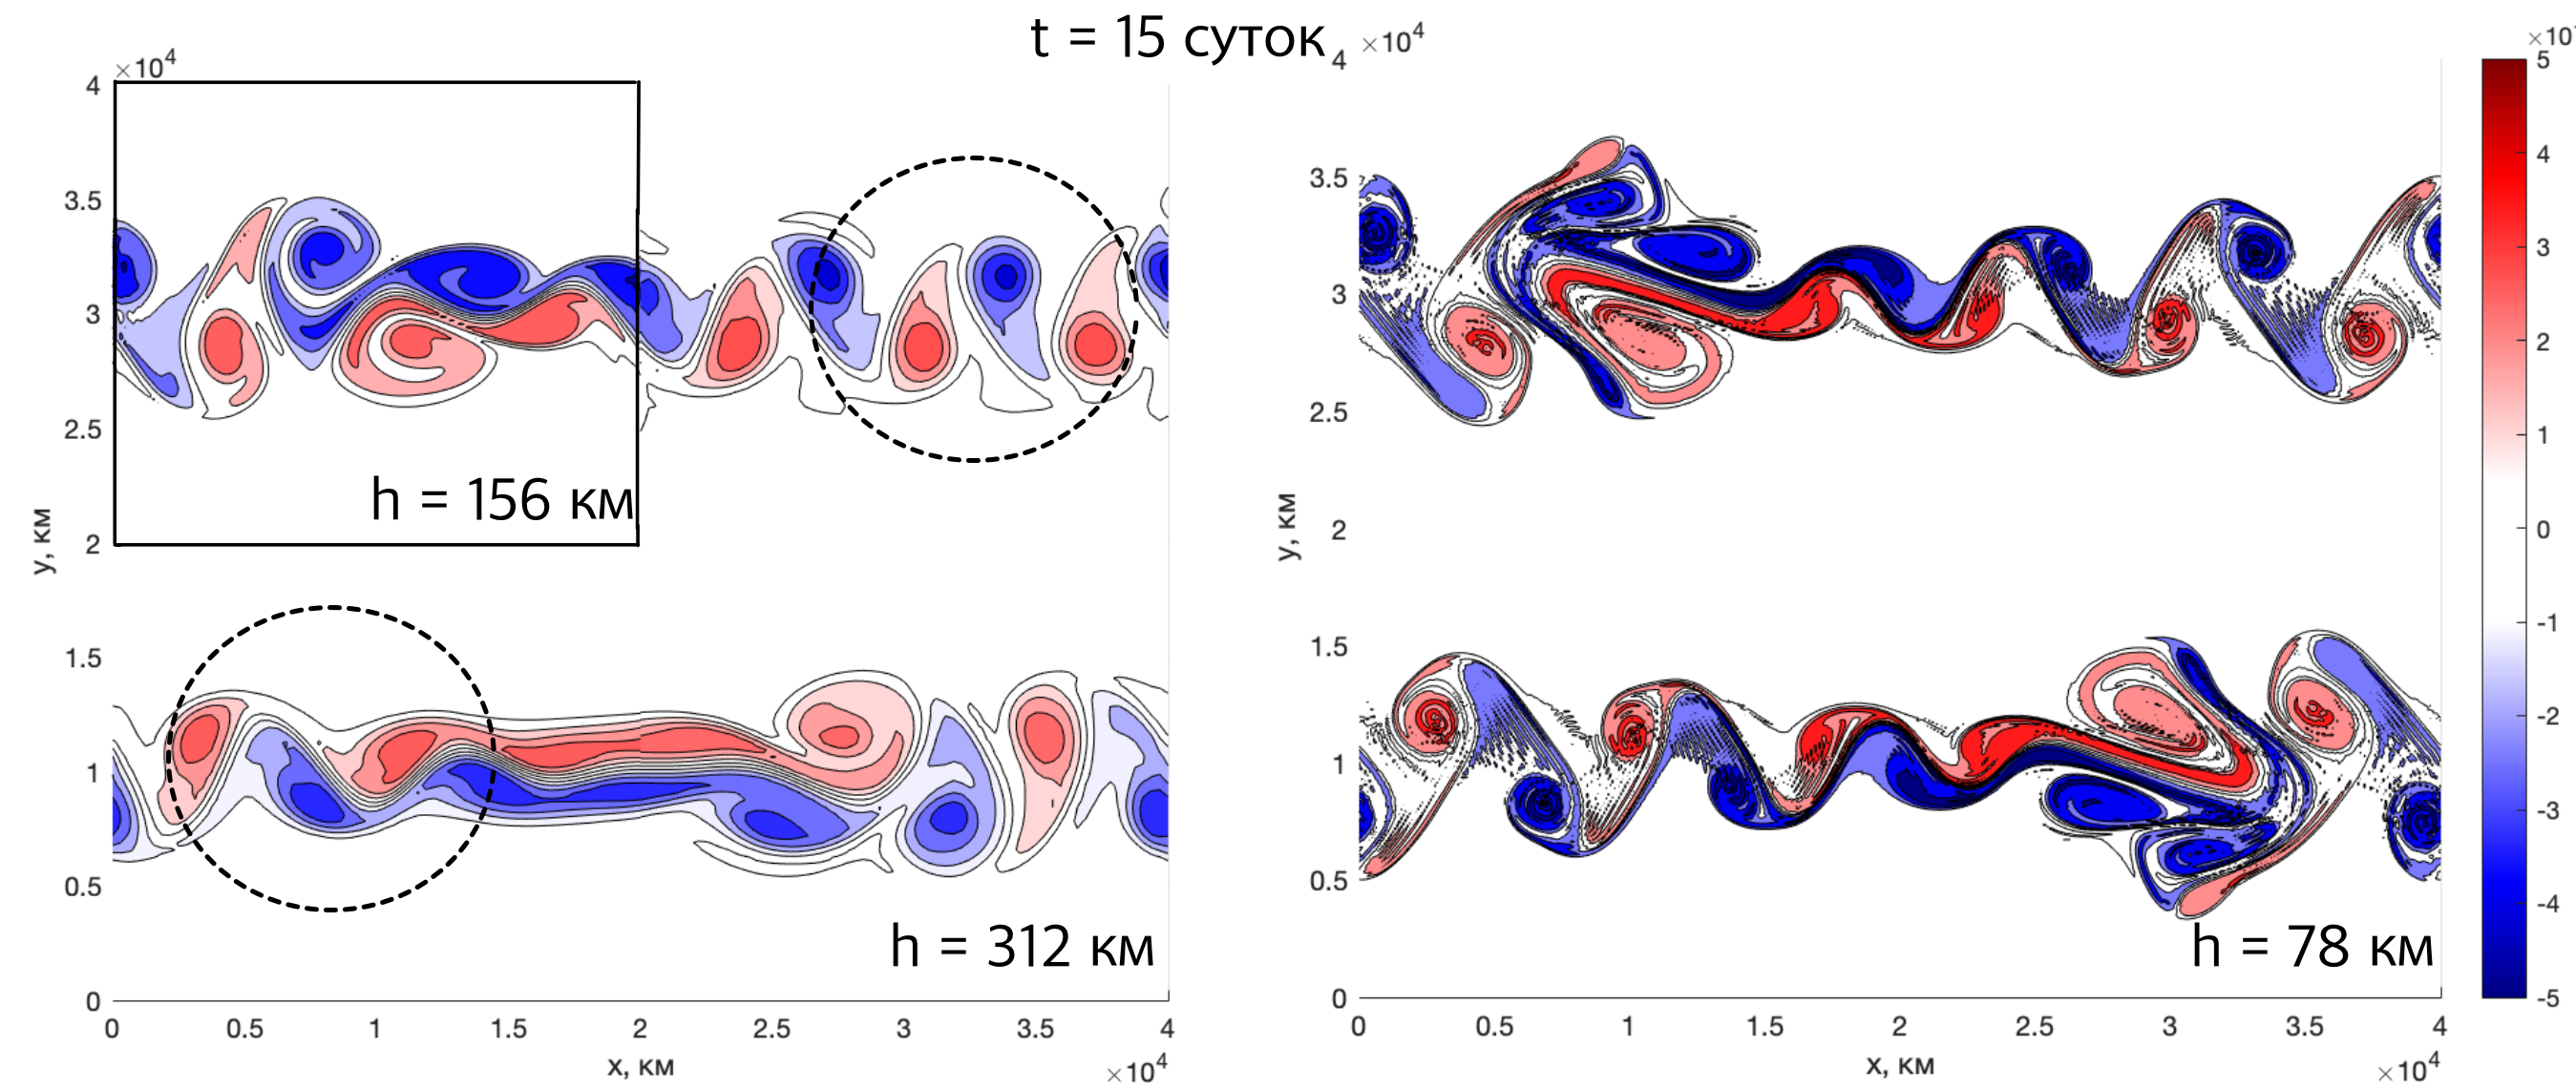
\includegraphics[width=1\linewidth]{./images/kelhelm15.png}
\caption{Relative vorticity field after 15 days}
\label{fig:mpr}
\end{figure}
\end{frame}


\begin{frame}{Conclusion}

An approach based on the SAP-SAT method for approximating shallow water equations on grids with local refinement is proposed.

\textbf{Approach advantages}
\begin{enumerate}
\item Mass and energy conservation
\item Stability, a proven theorem
\item High-order of approximation
\item Local refinement has a positive impact on entire solution as a whole
\end{enumerate}

\textbf{Approach disadvantages}
\begin{enumerate}

\item Approximation orders reduction near block boundaries
\end{enumerate}

\end{frame}

\begin{frame}{Further research}

\begin{enumerate}
\item Approach implementation within spherical geometry
\item Approach implementation for three-dimensional equations of atmospheric dynamics
\item Comparison with other methods

\end{enumerate}

\end{frame}

\begin{frame}
\center{\huge{Thanks for your attention}}
\begin{figure}[h]
\centering
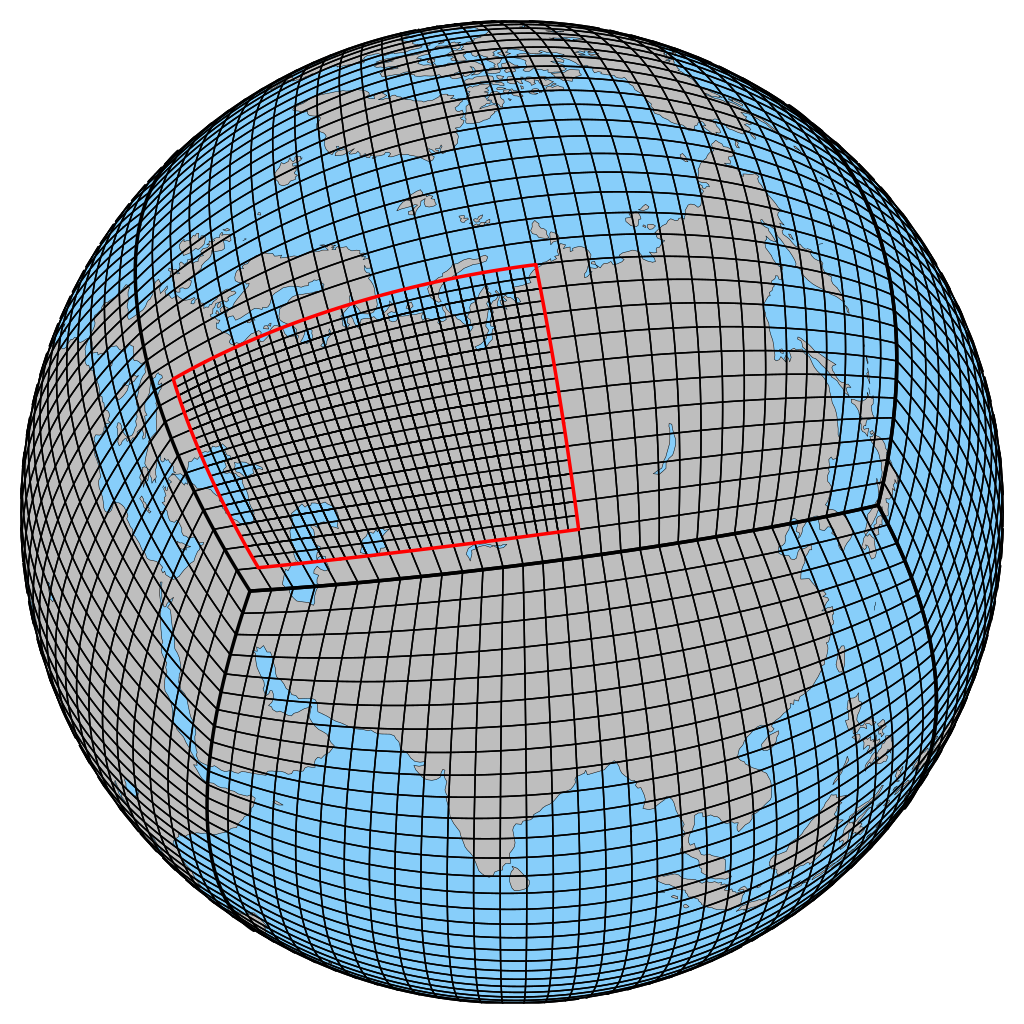
\includegraphics[width=0.4\linewidth]{./images/cubsphere.png}
\end{figure}
\end{frame}

\end{document}